\section{The Hilbert's theorem}
\begin{theorem}[Hilbert's theorem]
    Let \(S\) be a complete and simply connected regular surface with
    Gaussian curvature \(K=-1\), then there is no isometric embedding of
    \(S\) into \(\mathbb{R}^3\).
\end{theorem}
\begin{proof}[Sketch of proof]
    \begin{enumerate}[(1)]
        \item \((S,g)\) is isometric to the hyperbolic plane in 
        \(\mathbb{H}^2\)\\
        \(\Rightarrow\) \(Area(S)=Area(\mathbb{H}^2)=+\infty\).
        \item If \(\exists\) an isometric embedding \(
            \varphi\colon S\to \mathbb{R}^3\), then we can construct a 
            global parametrization of \(S\) with coordinate curves being
            asymptotic lines, and the parametrization forms a
            ``chebyshev net'' such that any quadrilateral of coordinate
            curves has area \(<2\pi\). This implies 
            \[Area(S)<2\pi.\]
    \end{enumerate}
    Then (1) and (2) yields a contradiction.
\end{proof}
\begin{definition}
    A local parametrization \(\phi (u,v)\colon U\subset \mathbb{R}^2\to
    S\) is called a ``chebyshev net'' if the length of opposite sides of
    any quadrilateral formed by coordinate curves are equal.
\end{definition}
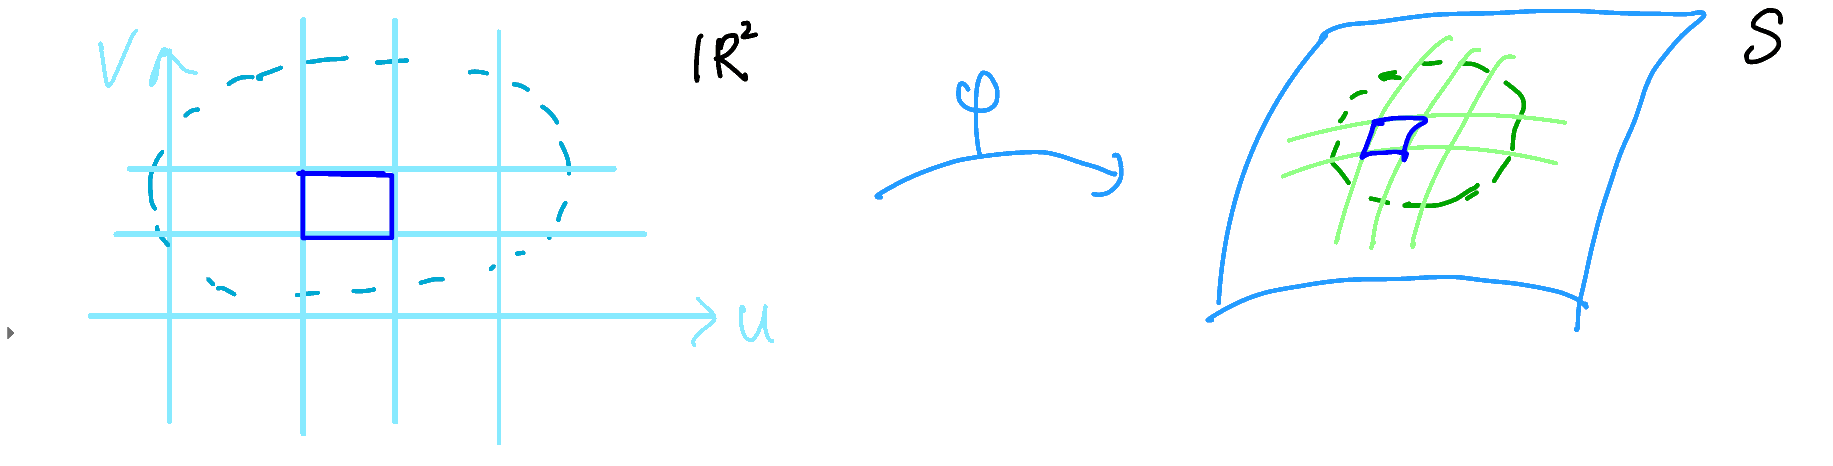
\includegraphics[scale=0.4]{picture/week15/chebyshev net.png}
\begin{proof}[proof of (1)]
    First, from the minding's theorem, we know \(S\) and \(\mathbb{H}\)
    are locally isometric to each other. Let \(p\in S\), \(p'
    \in \mathbb{H}\), the local isometry yields a linear isometry
    \(l\colon T_p S\to T_{p'} \mathbb{H}\).

    To construct a global isometry, let's consider
    \begin{center}
        \begin{tikzcd}
            T_p S \arrow[d, "\exp_p"] \arrow[r, "l"] & T_{p'}\mathbb{H} \arrow[d, "\exp_{p'}"] \\
            S \arrow[r, dashed]                      & \mathbb{H}                             
        \end{tikzcd}
    \end{center}
    By the Hadamard theorem \(\rightarrow\) \(\exp_p\) and \(\exp_{p'}\)
    are diffeomorphism.
    \footnote{
        Hadamard's theorem: let \((M,g)\) be a complete Riemannian manifold
        with \(K_M\le 0\), where \(K_M\) is the sectional curvature, then
        \(\exp_p\colon T_p M\to M\) is a covering map. Moreover, if \(M\)
        is simply connected, then \(\exp_p\) is a diffeomorphism.
    }
    Hence \(f=\exp_p\circ l\circ \exp_{p'}^{-1}\colon S\to \mathbb{H}\)
    is a diffeomorphism. We can further conclude that \(f\) is a local 
    isometry. This follows from the Cartan's theorem:
    \begin{itemize}
        \item Let \((M,g)\), \((M',g')\) be two Riemannian manifolds, 
        \(p\in M\), \(p'\in M'\).
        \item Let \(l\colon T_p M\to T_{p'}M'\) be a linear isometry
        \item \(U\) is a normal neighborhood of \(p\) on which \(\exp_p\)
        is a diffeomorphism.
        \item \(\forall V\in T_q M\), and let \(P_t\) be the parallel transport
        along \(\gamma(t)\), then \(P_t^{-1}(V)\) is a vector in \(T_p M\).
        The linear isometry yields \(l\circ P_t^{-1}(V)\) to be a vector
        in \(T_{p'}M'\). Let \(q'=\exp_{p'}\circ l\circ\exp_{p}^{-1}q
        \in M'\), \(\gamma'(t)\) is the geodesic from \(p'\) to \(q'\)
        and \(P_t'\) is the parallel transport along \(\gamma'(t)\).
        Then using \(P_t '\), we get a vector \(P_t'\circ l\circ 
        P_t^{-1}(V)\\in T_{q'}M'\)
        \(\Rightarrow L_t=P_t'\circ l\circ P_t^{-1}\colon T_q M\to
        T_{q'}M'\) is a linear isometry. If \(\forall\) vectors 
        \(X, Y,Z,W\in T_q M\) we have
        \[
            R(X,Y,Z,W)=R'(L_t(X),L_t(Y),L_t(Z),L_t(W))    
        \]
        then \(f=\exp_{p'}\circ l\circ \exp_p^{-1}\) is a local isometry.
        \begin{center}
            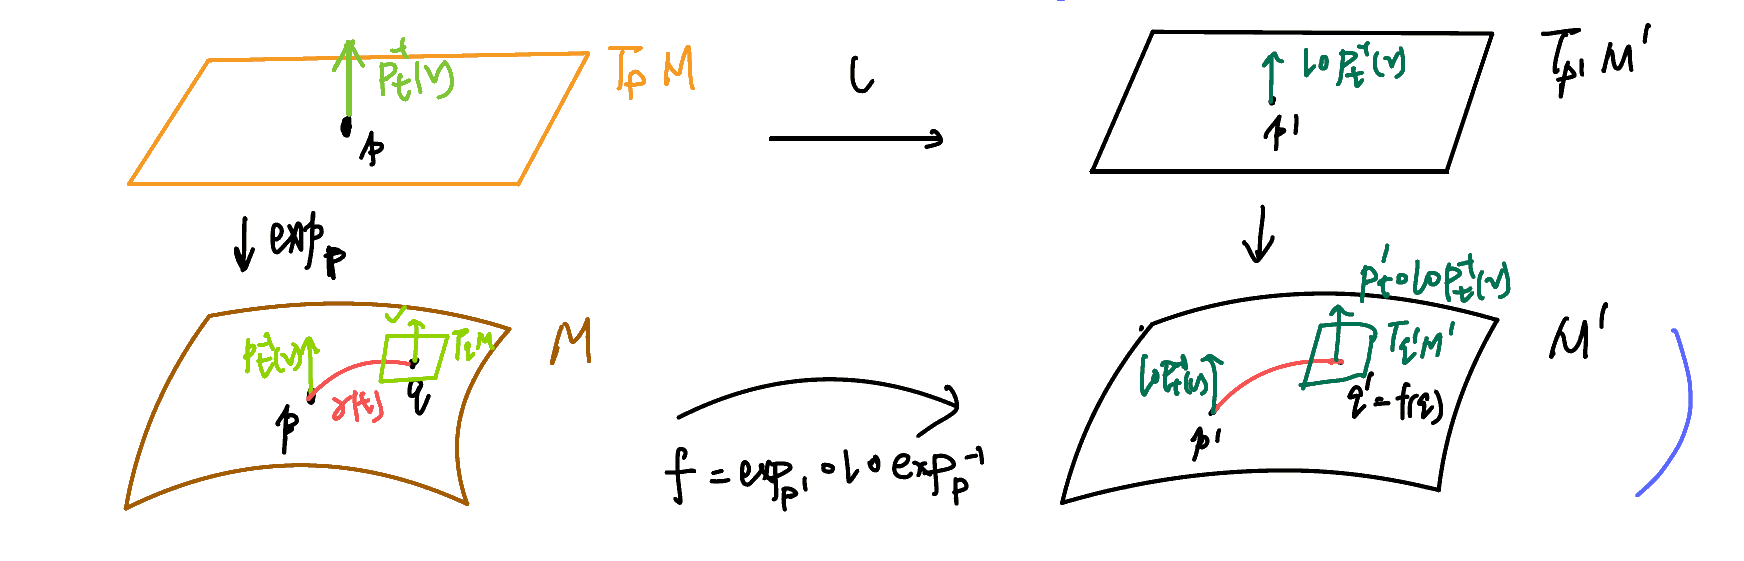
\includegraphics[scale=0.4]{picture/week15/cartan theorem.png}
        \end{center}
    \end{itemize}
    Hence, we see \((S,g)\) and \(\mathbb{H}\) are isometric to each other on
    \(\mathbb{H}^2\). We consider geodesic polar coordinate such that
    \[ds^2=dr^2+\left(\sinh r\right)^2 d\theta^2.\]
    Then the radial geodesic \(\gamma(t)=\exp_p(t\pdv{r})\) defines for all
    time \(t\), \(\Rightarrow t\in (0,+\infty)\)
    \[Area(S)=Area(\mathbb{H})=\int_{0}^{2\pi} \int_{0}^{+\infty}
    \sinh r drd\theta=+\infty\]
\end{proof}
\begin{proof}[proof of (2)]
    Now we assume \(S\) is isometrically embedded into \(\mathbb{R}^3\).

    \underline{Claim 1}: \(\forall p\in S\), \(\exists\) local parametrization
    \((s,t)\) of \(S\), such that the \engordnumber{1} and 
    \engordnumber{2} fundamental form are given by
    \[
      I=ds^2+2\cos \alpha ds dt +dt^2  
    \]   
    \[\II=2\sin\alpha ds dt\]
    where \(\alpha=\alpha(s,t)\) satisfies the Sine-Gordan equation
    \[\alpha_{st}=\sin \alpha,\quad 0<\alpha<\pi\]
    From this expression of I and II, we see
    \begin{enumerate}[(1)]
        \item the length of opposite sides of coordinate quadrilateral
        are the same \(\Rightarrow\) \((s,t)\) forms a chebyshev net,
        \(\alpha\) is the angle between \(s\)-curve and \(t\)-curve.
        \begin{center}
            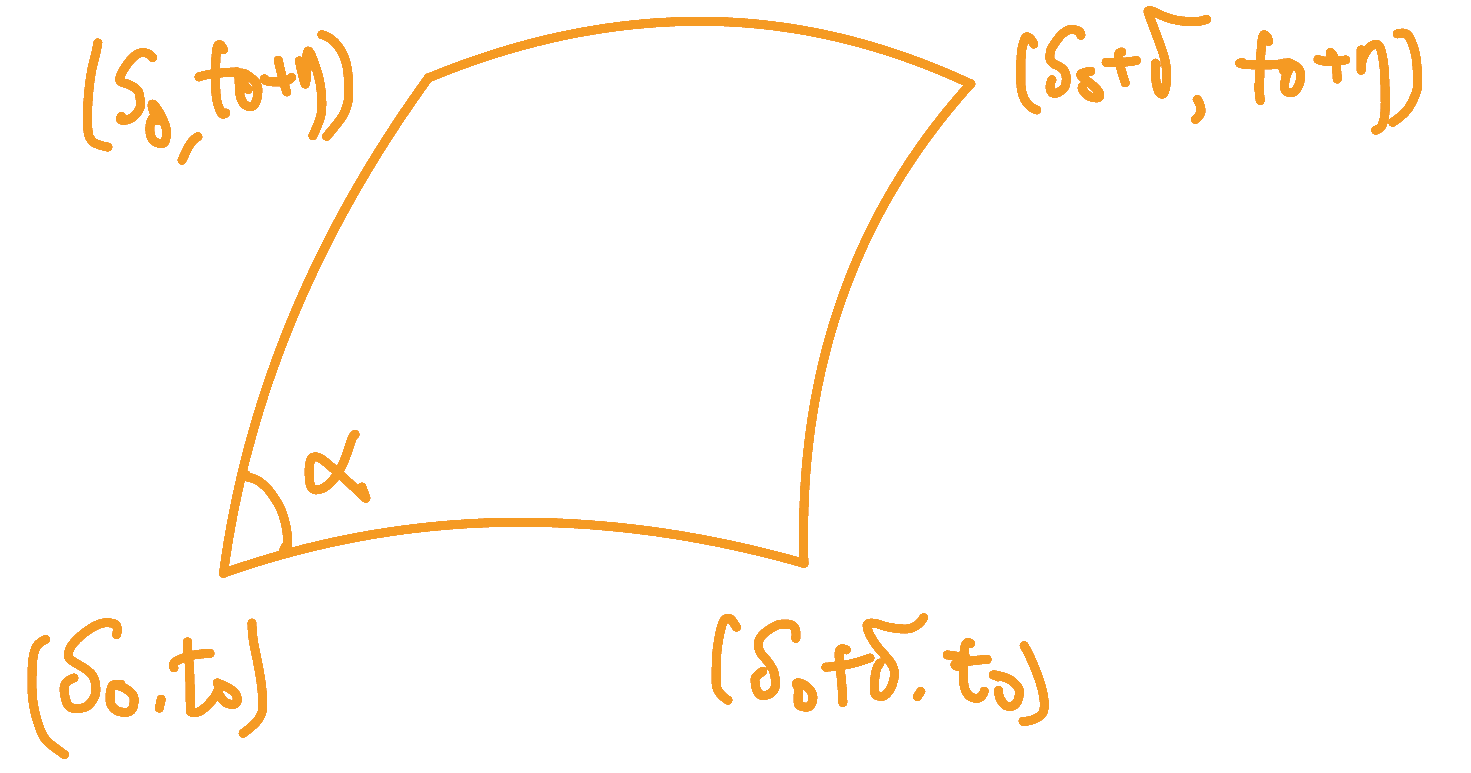
\includegraphics[scale=0.2]{picture/week15/quadrilateral.png}
        \end{center}
        \item coordinate \(s\)-curve and \(t\)-curve are asymptotic lines
    \end{enumerate}
    \begin{proof}[Proof of claim 1]
        \(K=-1\) on \(S\) \(\Rightarrow\) all pairs are umbilical.
        Hence, we can first choose local parametrization \(x^1,x^2\)
        such that 
        \[I=g_{11}(dx^1)^2+g_{22}(dx^2)^2\]
        \[II=h_{11}(dx^1)^2+h_{22}(dx^2)^2\]
    \(\Rightarrow\) principal curvatures \(k_1=\frac{h_{11}}{g_{11}},
    k_2=\frac{h_{22}}{g_{22}}\).
    The codazzi equation is 
    \[\frac{\partial_2k_1}{k_2-k_1}=\partial_2 \log \sqrt{g_{11}}\]
    \[\frac{\partial_1k_2}{k_1-k_2}=\partial_1 \log \sqrt{g_{22}}\]
    Since \(k_1k_2=-1\), we set 
    \[
        k_1=\tan\theta,\quad k_2=-\cot\theta,\quad 0<\theta<\frac{\pi}{2}    
    \]
    \(\Rightarrow k_1-k_2=\tan\theta+\cot \theta=
    \frac{1}{\sin\theta\cos\theta}\).
    Then the codazzi equation
    \begin{align*}
        \partial_2\log \sqrt{g_{11}}&=-\sin\theta\cos \theta
        \partial_2(\tan \theta)
        =-\sin\theta\cos\theta \frac{\cos\theta\partial_2\sin\theta
        -\sin\theta\partial_2\cos\theta}{\cos^2\theta}\\
        &=-\sin\theta\partial_2\sin\theta+\frac{1-\cos^2\theta}{\cos\theta}
        \partial_2\cos\theta\\
        &=-\partial_2\left(\frac{1}{2}\sin^2\theta+\frac{1}{2}
        \cos^2\theta\right)+\frac{\partial_2\cos\theta}{\cos\theta}
    \end{align*}
    \(\Rightarrow\partial_2 \left(
        \frac{\sqrt{g_{11}}}{\cos\theta}
    \right)=0\)
    Similarly, \(\partial_1\left(\frac{\sqrt{g_{22}}}{\sin\theta}\right)=0\)
    This enables us to introduce new coordinate
    \[
        y^1=\int    \frac{\sqrt{g_{11}}}{\cos\theta}dx^1\quad
        y^2=\int  \frac{\sqrt{g_{22}}}{\sin\theta} dx^2.
    \]
    \[
        dy^1=    \frac{\sqrt{g_{11}}}{\cos\theta}dx^1\quad
        dy^2= \frac{\sqrt{g_{22}}}{\sin\theta} dx^2
    \]
    \(\Rightarrow\) the \engordnumber{1} and \engordnumber{2} fundamental form
    in terms of \((y^1,y^2)\) are 
    \[
        I=\cos^2\theta (dy^1)^2 +\sin^2\theta(dy^2)^2 \quad
        II=k_1\cos^2\theta (dy^1)^2+k_2\sin^2\theta (dy^2)^2  
        =\sin\theta\cos\theta \left((dy^1)^2-(dy^2)^2\right)
    \]
    We consider further coordinate change. Let \(y^1=s+t,y^2=s-t\)
    \(
        (dy^1)^2=ds^2+dt^2+2ds dt
        (dy^2)^2=ds^2+dt^2-2ds dt    
    \)
    \(\Rightarrow \)In \((s,t)\) coordinate, the \engordnumber{1}
    and \engordnumber{2} fundamental form are 
    \[
        I=ds^2+2\cos 2\theta ds dt +dt^2    
    \]
    \[
        II=2\sin 2\theta ds dt    
    \]
    Let \(\alpha=2\theta\), then 
    \[
        I=ds^2+2\cos \alpha ds dt +dt^2    
    \]
    \[
        II=2\sin\alpha ds dt    
    \]
    Furthermore, from the Gauss equation, in \(y^1,y^2\) coordinate,
    \[
        I=\cos^2\theta (dy^1)^2 +\sin^2\theta (dy^2)^2   
    \]
    \begin{align*}
        K&=-\frac{1}{\sin\theta \cos\theta }\left(
            \partial_1\left(\frac{\partial_1\sin\theta}{\cos\theta}\right)
            +\partial_2\left(\frac{\partial_2\cos\theta}{\sin\theta}\right)
        \right)\\
        &=-\frac{1}{\sin\theta\cos\theta}\left(
            \pdv[2]{\theta}{(y^1)}-\pdv[2]{\theta}{(y^2)}
        \right)
    \end{align*}
    \[K=-1\Leftrightarrow \theta_{11}-\theta_{22}=\sin\theta\cos\theta
    =\frac{1}{2}\sin 2\theta \tag{1}\]
    \end{proof}
    \underline{Claim 2}: Any quadrilateral formed by coordinate courves
    in the chebyshev net on \(S\) has Area less that \(2\pi\)
    \begin{proof}
        If \((s,t)\) forms a chebyshev net, then 
        \[
            I=ds^2+2\cos\alpha ds dt+dt^2    
        \]
        with \(\alpha_{st}=\sin\theta\)(\(\because K=-1\)).

        Let \(\theta\) be the quadrilateral formed by coordinate curves,
        then 
        \begin{align*}
            Area(\theta)&=\int_{s_0}^{s_0+\delta}\int_{t_0}^{t_0+\eta}
            \sin \alpha ds dt \\
            &=\int_{s_0}^{s_0+\delta}\int_{t_0}^{t_0+\eta} \alpha_{st}ds dt\\
            &=\alpha(s_0+\delta,t_0+\eta)-\alpha(s_0+\delta,t_0)
            -\alpha(s_0,t_0+\eta)+\alpha(s_0,t_0)\\
            &<2\pi\quad(\because 0<\alpha<\pi)
        \end{align*}
    \end{proof}
    So far, we have shown \(\forall p\in S\), we have local parametrization
    \((s,t)\) near \(p\) such that \((s,t)\) forms a chebyshev net and 
    coordinate curves are asymptotic curves.

    In fact, we can establish a global parametrization on \(S\), which
    forms a chebyshev net and coordinate curves are asymptotic curves
    in the following way.

    Let's first define such global parametrization:
    \[
        \varphi\colon \mathbb{R}^2 \to S   
    \]
    Take a point \(p\in S\), let \(\alpha_1,\alpha_2\) be asymptotic curves
    through \(p\). Let \(p\) be corresponding to the origin \((0,0)\)
    in \(\mathbb{R}^2\). For each \((s,t)\in\mathbb{R}^2\), we consider
    \(\varphi(s,t)\in S\) to be found in the following way. We first
    find a point \(p_1\) along \(\alpha_1\) with distance \(s\) from 
    \(p\). At \(p_1\) we can still choose \(\alpha_1\) as asymptotic line.
    (by the uniqueness of differential equation \(II(\alpha'(s),\alpha'(s))\))
    Since \(p_1\) is again a hyperbolic point, we have another asymptotic curve
    \(\alpha_2\) which is obtained by continuous extending
    \(\alpha_2\) along \(\alpha_1\). Along this \(\alpha_2'\),
    choose point \(p_2\) with distance \(t\) from \(p_1\).
    Let \(\varphi(s,t)=p_2\in S\).

    In this way, we define a map 
    \[
        \varphi\colon \mathbb{R}^2\to S
    \]
    \[(s,t)\mapsto \varphi(s,t)\in S\]
    There are a few things to be checked.
    \begin{enumerate}[(1)]
        \item \(\varphi(s,t)\) is well-defined for all \((s,t)\in 
        \mathbb{R}^2\)

    (Here we need to use the completeness of \(S\). 
    If \(\varphi(s,t)\) is not defined for some
    \(\sigma=s_1\),\ie\ the asymptotes curve \(\alpha_1\) 
    is defined on \(\left[0,s_1\right)\), let \(
      q=\lim_{s\to s_1}\alpha_1(s)  
    \) by the
    completeness of \(S\) , \(q\in S\). 
    Hence, we can establish a local parametrization 
    given by chebyshev net
    with coordinate curves being asymptotic curves. 
    Hence, \(\varphi(s,0)\) is defined similarly for any
    fixed \(s\). \(\varphi(s,t)\) is defined for all t.)
    \item For any fixed \(t\), \(\varphi(s,t)\) is an asymptotic
    curve with \(s\) being the arclength.

    (First, for any \(\varphi(s',t')\in S\), we can find a 
    ``rectangular'' coordinate chart \(s_a<s<s_b, t_a<t<t_b\)
    such that \(\varphi(s,t)\) forms a chebyshev net with coordinate 
    curves being asymptotic curves. 
    By the definition of \(\varphi(s,t)\), if for any \(t_0\in 
    (t_a,t_b)\), \(\varphi(s,t_0)\) is an asymptotic curve, so 
    for any \(t\in (t_a,t_b)\), \(\varphi(s,t)\) is an asymptotic curve.

    Second, let \(\varphi(s_1,t_1)\in S\) be arbitrary point,
    \(\varphi(s_1,t),0\le t\le t_1\) is a compact segment, we can
    cover it by finitely many rectangular neighborhoods and each of
    them is a chebyshev net. Since \(\varphi(s,0)\) is an asymptotic
    curve we can iterate the previous step to see \(\varphi(s,t)\)
    is an asymptotic curve.)
    \item \(\varphi(s,t)\colon \mathbb{R}^2\to S\) is a diffeomorphism.
    \begin{itemize}
        \item \(\varphi(s,t)\) is a local diffeomorphism.(easy to see)
        \item \(\varphi\) is injective.
        \item \(\varphi\) is surjective, we shall see otherwise this would
        contradics the completeness. 
        If \(\varphi(\mathbb{R}^2)=U\neq S\), then \(U\) has nonempty
        boundary \(\partial U\)
        \begin{center}
            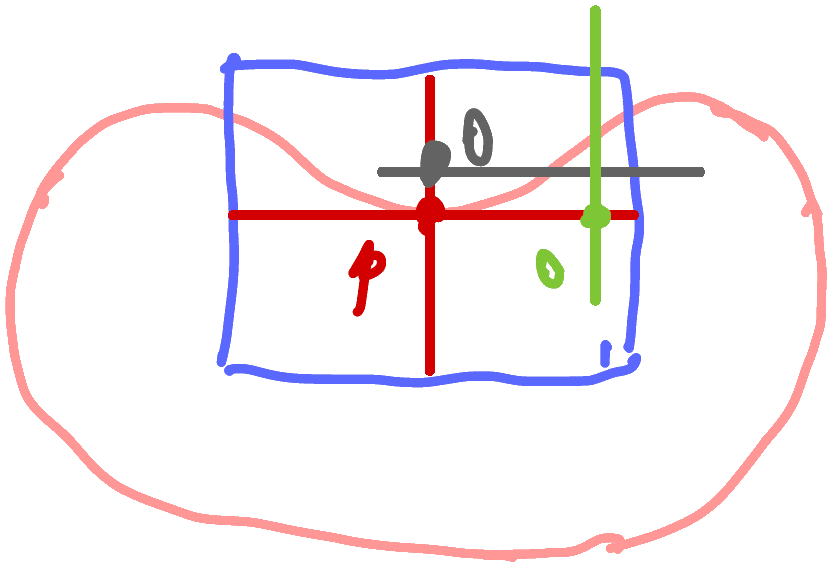
\includegraphics[scale=.4]{picture/week15/surjectiveness.png}
        \end{center}
        If \(\varphi(\mathbb{R}^2)=U\neq S\), then U
        has nonempty boundary \(\partial U\)
        \item Let \(q\in \partial U\), since \(p\in S\), we have local 
        chebyshev net \(R\) at \(p\). In \(R\), each coordinate line 
        is an asymptotic curve.
        
        \item Take \(q\in U\cap R\), then one of the asymptotic curve
        (coordinate curve) of \(q\) (green or grey line) will meet with
        an asymptotic coordinate curve of \(p\)(red lines) at some point
        \(o \in S\). The chebyshev net of \(o\) can be chosen to be contained
        in the intersection of chebyshev nets of \(p\) and \(q\)
        \begin{enumerate}[(1)]
            \item If \(o\in U\), since \(\varphi(\mathbb{R}^2)\)
            is the largest extension of chebyshev net, and \(p\notin U\).
            This implies asymptotic coordinate curves of \(o\)
            can not pass through \(p\) (contradiction)
            \item If \(o\notin U\), then asymptotic coordinate line 
            of \(o\) can not pass through \(q\), otherwise \(q\notin U\)
            (contradiction).
        \end{enumerate}
    \end{itemize}
    \end{enumerate}
\end{proof}
\begin{remark}
    In the proof of Hilbert's theorem, we have used a fact that
    the isometric embedding \(f\colon S\to \mathbb{R}^3\) is at least
    \(C^3\)(since we need this to compute I,II and codazzi equation).
    Efimov showed there is no \(C^2\) isometric embedding.
    There is a counterexample due to Kuiper in 1955, showing that
    one can find \(C^1\) isometric embedding \(f\colon U^+\to
    \mathbb{R}^3\), where \(U^+=\) upper half plane with metric
    \(\frac{dx^2+dy^2}{y}\)
\end{remark}